\documentclass[draft, a4paper, abstract=on]{scrartcl}

%section{ignore warnings}

  \usepackage{silence}
  \WarningFilter{latex}{Marginpar on page}

%section{packages}

  \usepackage{packages}
  \addbibresource{~/promo/bib/references.bib}
  \usepackage{url}

%section{new commands}

  \renewcommand{\hw}[1]{\textbf{#1}}

  \newcommand{\lsil}[1]{\lstinline[language=Python]{#1}}
  \newcommand{\mtrc}[1]{\textcolor{blue}{#1}}

  \newcommand{\sw}[1]{\texttt{#1}}

\begin{document}
%section{title}

  \title{Social networks of lexical innovation}
  \subtitle{Investigating the diffusion of neologisms on Twitter}
  \author{Quirin Würschinger\\ LMU Munich}
  \maketitle

%section{todos}

\listoftodos

%section{abstract}
  \cleardoublepage

  \begin{abstract}

    Societies continually evolve and speakers coin and use new words to talk about innovative products and practices. While most lexical innovations fail to catch on, others spread successfully and become part of the lexicon. This paper investigates the diffusion of English neologisms on Twitter. Previous work on lexical innovation has almost exclusively relied on usage frequency counts for measuring diffusion. Taking frequency as a baseline, we use social network analysis to zoom in on the sociolinguistic dynamics of diffusion.

    Our results show that frequency counts lend themselves to approximate overall degrees of diffusion with varying success. While absolute counts can be misleading, incorporating temporal dynamics of use provides a better picture of diffusion. However, frequency-based information alone fail to capture important sociolinguistic characteristics. Social network information are shown to add valuable information about whether new words are known and used by an increasing number of individuals and communities of speakers. Firstly, we distinguish different pathways of diffusion depending on whether and to which degree new words show increasing vs. decreasing centralized use over time. Secondly, we show that social network information allow for more fine-grained assessments of degrees of diffusion, for example when new words are used with increasing frequency while their remains limited to certain parts of the speech community. Lastly, we compare our results based on usage frequency and on social network analysis. Besides notable discrepancies, we find a significant correlation between both types of information which serves to cross-validate both approaches.

    Our results suggest that social network information can complement frequency counts and that using information from both sources provides a more reliable and differentiated view of the sociolinguistic dynamics of diffusion. We suggest that this is particularly important for investigating the diffusion of lexical innovations, as new words are often marked by high social indexicality and show substantial differences in use between communities of speakers. More generally, however, social network analysis shows great potential to study sociolinguistic dynamics of language variation and change on all linguistic levels.


    \vspace{2\baselineskip}

    \textbf{Keywords}: lexicology, lexical innovation, sociolinguistics, diffusion, social media, Twitter, big data, social network analysis

  \end{abstract}

% text body

\section{Introduction}

Societies continually evolve, new products and practices emerge, and speakers coin and adopt new words when they interact and share information. How do these new words spread in social networks of communicative interaction?

Covid-19 has recently spread through social contagion with shocking speed and has tragically affected the lives of people around the world. Its fatal consequences have demonstrated the devastating power of exponential diffusion in social networks. In a recent paper analysing contagion patterns of diseases in \emph{Nature Physics}, \textcite{Hebert-Dufresne2020MacroscopicPatterns} suggested that the spread of viruses follows principles of complex contagion through social reinforcement and that it matches the dynamics of diffusion of cultural and linguistic innovations such as new words and internet memes. Does this confirm the widespread perception that new words \enquote{go viral}?

Influential sociolinguistic models of the spread of linguistic innovations like the S-curve model~\parencite{Milroy1992LinguisticVariation} share fundamental features with earlier economic models~\parencite{Rogers1962DiffusionInnovations} of diffusion and show commonalities between the spread of cultural and linguistic innovations. These models assume that diffusion in social networks follows universal trajectories and that rates of spread depend on social dynamics such as network density and the presence or absence of weak ties~\parencite{Granovetter1977StrengthWeak}. Unlike research on biological and cultural diffusion processes, however, sociolinguistic research has only recently been provided with data sources that are equally suitable for large-scale, data-based approaches using social network analysis to study these phenomena empirically.

Social media platforms like Twitter have changed the way we communicate and how information spreads, and they offer large amounts of data for empirical research. Sociological research has been concerned with pressing issues regarding the impact of online social networks for the spread of hate speech, fake news and the power of \enquote{influencers}, bots and institutions on public opinions and elections, which increasingly strain the social fabric. For (socio-)linguists, social media provide large amounts of data of authentic language use which opens up new possibilities for the empirical study of language variation and change. The size of these datasets as well as their informal nature allow for large-scale studies on the use and spread of new words, for example, to gain insights about general trajectories~\parencite{Nini2017ApplicationGrowth} or about factors that influence whether new words spread successfully~\parencite{Grieve2018NaturalSelection}. Moreover, metadata about speakers allows studying aspects of diffusion that go beyond what can be captured by usage frequency alone. Recent work has, for example, used Twitter data to investigate the geographical spread of lexical innovations.~\parencite{Eisenstein2014DiffusionLexical,Grieve2017GeographicalPatterns,Grieve2018MappingLexical}

Data about the communicative interaction of speakers additionally allows performing network analyses of the social dynamics of diffusion processes. Network science approaches to social media data have been successfully employed in diverse fields, for example, to study the spread of diseases~\parencite{Lu2018AccurateInfluenza}, opinions~\parencite{West2014ExploitingSocial} and political attitudes~\parencite{PewResearchCenter2019NationalPolitics}. While the study of social networks has a long research tradition in sociolinguistics and has shaped influential models of diffusion~\parencite[e.g.][]{Milroy1985LinguisticChange}), large-scale network analyses of sociolinguistic phenomena have only recently become more widespread. These new data sources and methodological advances put computational sociolinguistics in an excellent position to gain new insights and to test long-standing theoretical models empirically.

In the area of lexical innovation, this can serve to evaluate important theoretical concepts like the role of early adopters, network density and weak ties in the diffusion of new words. For example, earlier approaches have used computational modelling to test the validity of the S-curve model~\parencite{Blythe2012ScurvesMechanisms}, and to model processes of simple and complex contagion of linguistic innovations in social networks~\parencite{Goel2016SocialDynamics}. Applying social network analysis to bigger samples of neologisms and tracking their diffusion on social media datasets promises to shed light on whether the adoption of new words remains limited to closely connected sub-communities or whether they reach larger parts of the speech community and whether individuals or groups drive this process.

This paper makes use of social media data and social network analysis to study the diffusion of lexical innovations on Twitter. Taking usage frequency as a baseline, we conduct a longitudinal study monitoring the use of a broad sample of neologisms to analyse their cumulated usage frequency as well as the temporal dynamics underlying their spread. We additionally conduct social network analyses of our neologism sample to get a better picture of the sociolinguistic dynamics at play to assess different pathways and overall degrees of diffusion. Lastly, we compare both approaches to assess their validity, and we combine information from both sources to draw a more differentiated picture of diffusion.

The paper is structured as follows. Section 2 presents an overview of previous attempts to modelling and measuring the diffusion of lexical innovations in order to contextualise and define the present theoretical framework and its operationalisation for the empirical study. Section 3 provides information regarding the present sample of neologisms and the collection and composition of the Twitter dataset this study is based on. Section 4 describes the methodological procedure for analysing diffusion in this dataset, focusing on the construction and analysis of social networks. Section 5 presents the empirical results obtained from using usage frequency and social network analysis to study diffusion, and from comparing both approaches. Section 6 summarises and discusses these results and suggests theoretical implications and directions for future work.

\section{Modeling the diffusion of lexical innovations}

Speakers continually coin new words, yet most fail to spread successfully and fall into oblivion. How do new words diffuse to be known and used by more and more speakers and to become conventional lexemes in a language system? And how can diffusion be modelled theoretically and measured empirically?

Neologisms are on a continuum from entirely novel word-formations to established lexemes that are familiar to the majority of the speech community. Neologisms have spread to some extent, but are still perceived as new or unknown by many speakers. On one end of the continuum, `nonce-formations' are new words that have been coined in a concrete communicative situation, but are not adopted by interlocutors to be used in future usage contexts and do not enter a process of continuous diffusion.~\parencite{Hohenhaus1996AdhocwortbildungTerminologie} Fully established words form the other end of the continuum. They are known and used by most or all members of the speech community and codified in dictionaries. This latter, lexicographic feature marks speakers' agreement on how these words are to be used and is a sign of their status as conventional lexical units in the language system.

Neologisms occupy an intermediate position between both poles and can be defined as

\blockquote[{\cite[31]{Kerremans2015WebNew}}]{
[\dots] lexical units, that have been manifested in use and thus are no longer nonce-formations, but have not yet occurred frequently and are not widespread enough in a given period to have become part and parcel of the lexicon of the speech community and the majority of its members.
}

Diffusion thus represents the process that transports successful neologisms along this continuum, becoming increasingly conventional in the speech community.

A more precise definition is provided by \citeauthor{Schmid2020DynamicsLinguistic}: \blockquote[\cite{Schmid2020DynamicsLinguistic}]{I define diffusion as a process that brings about a change in the number of speakers and communities who conform to a regularity of co-semiotic behaviour and a change in the types of cotexts and contexts in which they conform to it.} \todo{page?}

this definition includes three dimensions of diffusion

  cotext
  context
  speakers

i will focus on sociolinguistic dimension in this paper
  spread across
    speakers
    communities

previous work has taken at
  structural and
  cognitive perspectives

i will focus on the sociolinguistic perspective

most relevant and important model: S-curve model

  \subsection{Research perspectives}

  A substantial body of linguistic research has tackled this question from different \hw{perspectives}. \parencite[16]{Schmid2016EnglishMorphology}

  From a \hw{structural} perspective, main areas of interest include which word-formation processes are involved in forming new words, whether they are formally and semantically transparent, whether they change in the process of lexicalization and which status the resulting neologisms have in the language system (institutionalization). \parencite[e.g.][]{Bauer1983EnglishWordformation, Lipka2005LexicalizationInstitutionalization}

  \hw{Cognitive} perspectives focus on how individuals process and store lexical innovations. Speakers generally use new words when they experience a communicative need to talk about entities or practices that cannot be expressed by their language's inventory of conventional words yet. In order for neologisms to successfully diffuse, speakers need to successfully negotiate their meaning (co-semiosis) in discourse, others need to adopt the behaviour of using these words (co-adaption). Continued exposure and use of new words can then lead to the entrenchment of new words in the mental lexicon of speakers.~\parencite{Schmid2008NewWords}

  \hw{Sociolinguistic} perspectives transcend the level of the individual to study the diffusion of new words across speakers. The diffusion of lexical innovations is commonly seen as successful when the majority of the speech community has accepted a new word as a conventional lexical unit that can and is being used in communicative practice.


  \subsection{The S-curve model}

  \hw{S-curve models} of linguistic change~\parencite{Milroy1992LinguisticVariation, Nevalainen2015DescriptiveAdequacy, Labov2007TransmissionDiffusion} assume universal sociolinguistic dynamics for the diffusion of linguistic innovations.

  \begin{easylist}[itemize]

  # The \hw{trajectory} of spread is expected to follow an S-curve shape, with low rates of diffusion in early stages, followed by a period of accelerating spread with a tipping point at the mid point in the diffusion curve after which diffusion slows down and the curve flattens towards the end of the diffusion process.

  # These temporal trajectories are assumed to correspond to the \hw{sociolinguistic dynamics} of which individuals and groups interact with each other and adopt the target innovation.

  ## In the \hw{first stage} of slow diffusion only few early adopters take up the innovative words. The individuals who use the new word typically form dense networks connected by strong ties. The structure of tight-knit communities of potentially like-minded individuals of similar backgrounds facilitates the successful negotiation of meaning (co-semiosis) of new words. High rates of interactions in these communities leads to high rates of exposure for individuals, which fosters co-adaption, entrenchment and usualization of new words in these communities.

  ## In cases of successful diffusion the initial stages are followed by an \hw{acceleration in spread} when new words increasingly reach speakers outside these tight-knit communities via weak ties~\parencite{Granovetter1977StrengthWeak}. Rates of diffusion increase substantially when speakers that are not part of the initial group of early adopters start to accommodate the new words, allowing the innovations to reach a broader spectrum of the speech community.

  ## In \hw{later stages}, rates of diffusion slow down again as the majority of the speech community has already adopted the new words while smaller pockets speakers remain reluctant to take up the new words.

  # S-curve models have mainly been applied to the \hw{linguistic domains} of phonology and syntax. Fundamental differences between lexemes and linguistic items on other levels such as phonemes and grammatical constructions might affect the validity and reliability of such models for \emph{lexical} innovation.

  ## For example, grammatical constructions such as the \ol{going to} future used to express a speaker's future intention serve to fulfil relatively abstract communicative needs that remain stable over time. By contrast, on the lexical level, linguistic innovations are typically tied to concrete cultural referents such as products and practices whose conceptual relevance is much more volatile over time. For example, many lexical innovations such as \ol{millennium bug} denoting the fear of a computer crash at the beginning of the new millennium can show high rates of diffusion and become entrenched and conventional among the majority of the speech community. Without continual conceptual relevance in public discourse, however, these words fail pass on to the next generation of speakers. S-curves are commonly assumed to be found when linguistic innovations compete for \hw{\enquote{semantic carrying capacity}}~\parencite{Nini2017ApplicationGrowth}, however, in many if not most cases of \emph{lexical} innovation the conceptual carrying capacity is far from stable over time which represents a critical deviation from the traditional assumptions behind S-curves in language change.

  ## However, the generally strong theoretical and empirical basis of the S-curve model for language innovation and change, also from studies on the diffusion of cultural innovations~\parencite{Rogers1962DiffusionInnovations}, and the precise formulation of the sociolinguistic dynamics underlying different phases of diffusion still make it an attractive \hw{blueprint} for the empirical study of the sociolinguistic diffusion of lexical innovations.

  \end{easylist}


  \subsection{Current framework: the EC-Model (Schmid 2020)}

  I use the Entrenchment-and-Conventionalization-Model~\parencite{Schmid2020DynamicsLinguistic} as a framework for modelling the diffusion of lexical innovations.

  The EC-Model provides an approach integrating both structural, cognitive and sociolinguistic perspectives on the diffusion of lexical innovations.

  The model also differentiates between the level of the individual (\enquote{entrenchment}) and the community (\enquote{conventionalization}).

  Here I will only briefly outline the most important concept relevant for studying the sociolinguistic aspects of diffusion here.

  \hw{Conventionalization}:

  definition: \enquote{Conventionalization is the continual process of establishing and re-adapting regularities of communicative behaviour among the members of a speech community, which is achieved by repeated usage activities in usage events and subject to the exigencies of the entrenchment processes taking place in the minds of speakers.}~\parencite{Schmid2020DynamicsLinguistic}

  \hw{Usualization} \enquote{Usualization can therefore be defined as a process that establishes, sustains, and changes regularities of behaviour with regard to co-semiotic mappings between forms and meanings or functions and communicative goals and linguistic forms. It affects the semasiological, onomasiological, syntagmatic, cotextual, and contextual dimensions of conformity behind conventionality and is relative to communities.}~\parencite{Schmid2020DynamicsLinguistic}

  \hw{Diffusion} \enquote{Linking the three aspects of speakers, cotexts, and contexts, I define diffusion as a process that brings about a change in the number of speakers and communities who conform to a regularity of co-semiotic behaviour and a change in the types of cotexts and contexts in which they conform to it.}~\parencite{Schmid2020DynamicsLinguistic}

  less relevant for sociolinguistic aspects and for this study
  cotexts
  contexts

  According to the EC-Model, for studying the sociolinguistic aspects of diffusion, investigating \enquote{changes in the number of speakers and communities} is thus essential.

\section{Measuring the diffusion of lexical innovations}
  \subsection{Previous approaches}

  \begin{easylist}[itemize]

  # \hw{before frequency} Empirical approaches studying the diffusion of lexical innovations have only recently become feasible with the advent of new data sources and computational methods.

  # Earlier work had to rely on \hw{traditional linguistic corpora}. Due to the low-frequency nature of neologisms general linguistic corpora do not allow studying broad ranges of neologisms and thus pose limits to making broad and robust generalizations about the nature lexical innovation. Despite these limitations, case studies on selected neologisms~\parencite{Hohenhaus2006BouncebackabilityWebascorpusbased} and studies on specific domains of neology~\parencite{Elsen2004Neologismen} managed to shed light on the spread of new words in more specific domains.

  # The advent of \hw{web corpora} in the last two decades has provided researchers with bigger and less formal data to study lexical innovation.

  ## The sheer size of big corpora $\rightarrow$ bigger samples

  ## monitoring corpora~\parencite{Davies2013CorpusNews}: tracking dynamics of diffusion, closer to coining

  ## In particular, a range of tools enabled the creation of specialized corpora for the investigation of neologisms.~\parencite{Renouf2006WebCorpIntegrated, Kerremans2012NeoCrawlerIdentifying,LemnitzerWortwarte,Gerard2017LogoscopeSemiautomatic,Cartier2017NeoveilleWeb}

  ## the nature of web corpus data is particularly suitable for investigating lexical innovations as
  ### language on the web is very creative,
  ### more informal sources, bigger spectrum of language use
  ### new words often first occur on the web
  ### and use on the web significantly influences whether these new formations catch on or not.

  ## Web corpora thus promise insights into diffusion across
  ### contexts: e.g. whether new words such as \ol{blockchain} are increasingly used in less formal
  ### cotexts: e.g. whether new words such as \ol{} are increasingly used in more divers

  % # social media corpora \cite{Grieve2016AnalyzingLexical,Eisenstein2014DiffusionLexical}
  % ## size
  % ## nature: similar to web corpora
  % ### creative, hotbed
  % ### authentic language use
  % ### driving force
  % ## social network information

  % # \hw{social network analysis} getting at \enquote{changes in the numbers and communities of speakers} by using social network information
  % ## number of users: active and passive
  % ## interactions between users: influencers
  % ## network properties: density, centralization

  \end{easylist}

  \subsection{Going beyond frequency}

  The conventionality of linguistic units is commonly assessed by counting how often they are found to be used in linguistic corpora, with high frequencies of occurrence seen as indicators of high levels of conventionality. Diffusion as a process that drives increasing conventionalization is thus commonly assumed to be reflected by increases in the usage frequency of linguistic innovations. Previous research on lexical innovation has been largely limited to this approach and has evaluated the spread and the overall success of new words on the basis of the number of tokens found in linguistic corpora. This paper takes usage frequency as a baseline and uses social network analysis to go beyond frequency to discover sociolinguistic dynamics of diffusion and conventionality that have eluded previous frequency-based approaches.

  Frequency measures are widely used to study linguistic phenomena on all levels, from investigating phonological preferences between communities, to studying the increasing establishment of grammatical constructions like the \ol{going to}-future over time, to assessing the degree to which words are conventional lexical units of a language. Usage frequency is thus commonly used by a diverse set of linguistic sub-disciplines. From a structural perspective, for example, co-occurrence frequencies of multi-word units such as \ol{handsome man} are taken as an indicator for whether these are free combinations or more or less fixed collocations in a language system. Historical linguistics investigates phenomena like language change and grammaticalization, by analysing changes in usage frequency of certain constructions like the \ol{going to}-future over time. Cognitive and psycholinguistic research commonly relies on frequency measures to approximate the degree to which speakers are familiar with words that are presented as linguistic stimuli in experiments to control for effects on experimental results.

  The reliance on usage frequency as a measure for different phenomena in these diverse research contexts has faced substantial criticism. \cite{Stefanowitsch2017CorpusbasedPerspective} provide a good overview of the theoretical assumptions and problems that underlie frequency-based approaches in corpus linguistics.

  \todo{freq. esp. insufficient for lex. inn.}
  % as new words are
  (1) highly socially indexical and thus especially prone to be used only by certain sub-communities,
  (2) topical which makes freq. less reliable bc. it fails to capture \enquote{dormant} passive knowledge of the words

  When assessing the suitability of usage frequency as a measure for the diffusion and conventionality of neologisms a set of assumptions underlying the frequency-based approach need to be disentangled. While these theoretical and methodological considerations generally apply to all corpus-linguistic work, the focus will be on the current issue of lexical innovation.

  I adopt Schmid's EC-Model~\parencite{Schmid2020DynamicsLinguistic} as a framework for defining and delimitating the concepts of \enquote{conventionalization} and \enquote{diffusion}.

  \begin{quote}
  [\dots] I define diffusion as a process that brings about a change in the number of speakers and communities who conform to a regularity of co-semiotic behaviour and a change in the types of cotexts and contexts in which they conform to it.
  \end{quote}

  Aside from the sociolinguistic perspective on diffusion (\enquote{number of speakers and communities}), Schmid conceptualizes diffusion as a multi-dimensional process that also takes into account changes on the syntagmatic (\enquote{cotexts}) and pragmatic (\enquote{contexts}) level. This paper will focus on the sociolinguistic dimension of diffusion and will leave an integrative approach including all three perspectives for further research.

  Applying this definition to the context of lexical innovation thus implies that the successful diffusion of a new word is marked by it being known and used by an increasing \enquote{number of speakers and communities}.

  By contrast, in a strict sense, usage frequency counts of a lexeme represent the total number of tokens produced by \emph{all} speakers who have \emph{contributed} to the \emph{target text corpus}. The discrepancy between the theoretical definition of diffusion adopted here and the exact information contained by frequency show that this operationalization relies on a number of assumptions that let it only approximate the construct to be measured.

  Firstly, usage frequency does not provide direct information as to how many \emph{individual speakers} have used a new word. Especially in the case of neology, there are certain new words that are disproportionally used and propagated by a relatively small, but more active and dedicated users of the new term. This leads to high overall frequency counts which falsely suggest that larger parts of the speech community have adopted the term.

  Secondly, usage frequency only captures active uses of a term and fails to include how many speakers have been passively exposed to neologisms. In the context of entrenchment, \textcite{Stefanowitsch2017CorpusbasedPerspective} refer to this problem as the \enquote{corpus-as-input} and \enquote{corpus-as-output} hypothesis. The underlying assumption is that the output of the speakers who have contributed to a corpus can serve as an approximation for the potential linguistic input of a comparable speaker group. Frequency thus reflects the \enquote{usage intensity} of neologisms in the speech community which indicates the degree of entrenchment in individual speakers as well as an approximation of the conventionality of the neologisms in the speech community. In the case of lexical innovation this can be problematic as questionnaires studies on the use of neologisms~\parencite{Kerremans2015WebNew} show that many speakers report that they have come across target neologisms, but have not actively used them in discourse. Relying on frequency counts only can thus often lead to underestimating the degree of diffusion of neologisms.

  Thirdly, usage frequency fails to capture where new words diffuse across \enquote{communities of speakers}, as suggested by Schmid's definition. This is, of course, a consequence of the fact that frequency counts cannot provide direct information about the number of speakers involved in the diffusion of neologisms, as was pointed out in the first two points above. New words often stem and quickly spread within tight-knit communities of practice that share common attitudes or interests. Frequency measures alone cannot detect whether neologisms only show increasing usualization within these groups or whether they diffuse and become conventional in other parts of the speech community, which represents an essential feature of the sociolinguistic dimension of diffusion.


  how much the words might have diffused outside the \emph{target text corpus}

  temporal dynamics (e.g. \ol{millennium bug})


\section{Data}

  \subsection{Neologism sample}

    I base my empirical study on a selection of 100 neologisms and study their use on Twitter from the early stages of their diffusion to the end of 2018. The lexemes were selected to cover a broad spectrum of lexical innovation. Previous work by \textcite[115--147]{Kerremans2015WebNew} has identified four main clusters of neologisms on the conventionalization continuum: `non-conventionalization', `topicality or transitional conventionalization', `recurrent semi-conventionalization' and `advanced conventionalization`. My sample largely contains neologisms taken from the NeoCrawler, which uses dictionary-matching to retrieve a semi-automatic, bottom-up selection of recent neologisms on the web and on Twitter~\parencite{Kerremans2019UsingDatamining}. I have additionally included lexemes that were statistically identified as increasing in frequency on Twitter in recent years by \textcite{Grieve2016AnalyzingLexical}.



  dimensions

    overall degree of diffusion (synchronic): successful vs. unsuccessful: \mtrc{usage frequency}, \mtrc{degree centralization}
      no success
      limited
      advanced

    temporal dynamics of diffusion (diachronic)
      stability: stable vs. topical \mtrc{coefficient of variation}
      trend
      increasing: potential diffusion
      decreasing: potential centralization
      time window: speed and lifespan

    Case studies
      criteria
      covering clusters of neologism candidates
      frequency counts comparable
      cases~\parencite{Kerremans2015WebNew}
      no diffusion: \ol{microflat}
      limited
      topical: \ol{poppygate}
      centralized: \ol{alt-left}
      decreasing: \ol{solopreneur}
      advanced diffusion:
      advanced: \ol{upcycling}
      increasing: \ol{hyperlocal}



  \subsection{Twitter data}

  Twitter\footnote{\url{http://www.twitter.com}} is a popular micro-blogging and social media platform that was started in 2006.
  one of the most popular social media platforms

  representativity
  limited: certain user groups over-represented.
  good enough: generally okay \parencite{Grieve2019MappingLexical}

  advantages of data
  hotbed: influential hotbed for technical, cultural and linguistic innovations
  longitudinal: retrospective, starting from early attestations
  big data
  social network information

  scope of the present study:
  I only study diffusion of new words \emph{on Twitter}
  considering both frequency and social network characteristics might be more robust and allow more generalization than just frequency

  data retrieval
  I have used the tool \sw{twint}
  to download all tweets containing the target word
  as searchable via the Advanced Search Function on Twitter's official website

  data overview: table



\section{Method}

  anatomy of a tweet

  post-processing
    treatment of hashtags
    filter uses as user handles
    duplicate removal

  social network analysis
    software
      \sw{R}: \sw{tidygraph}, \sw{ggraph}
      \sw{Gephi}
    constructing the networks
      elements: legitimate~\parencite{Goel2016SocialDynamics}
      users = nodes
      interactions (replies, mentions) = edges
    subsetting: time slices
      start of diffusion process: >= 3 edges
      4 phases of equally sized time windows
    network metrics
      centralization
      network density
      visualizations

    result: interactional networks
      The resulting networks are interactional rather than static.~\parencite{Goel2016SocialDynamics} This makes them more similar to communities of practice than to traditional sociolinguistic networks based on static speaker characteristics such socio-economic status.
      In the case of lexical innovation networks that are based on whether speakers provide valuable information. In cases such as \ol{alt-left}, for example, interactional networks show whether usage of the term remains centralized to a tight-knit community of speakers or whether it diffuses to be used by other sub-communities.
      Whether communities are distinct depends on whether users communicate with each other. While the reasons for theses communicative affiliations remain unknown (age, gender, socio-economic status), they are certainly real in mutually engage in communicative interaction.
      It would be interesting to complement this information with static information, however such data are currently not obtainable.

\section{Frequency}

  \subsection{Total usage frequency}

  As described in Section XXX, the degree of conventionality is often approximated by a how many times a word has been used in a corpus. A common way to use this information is to rely on cumulated frequency counts which sum up the total number of uses.

  The present sample of neologisms covers a broad frequency range. Table \ref{tab:freq_total} presents candidates from four groups: six examples around the minimum, the median and the maximum total usage frequency as well as six words that will serve as case studies in the following sections.

  \begin{table}
  \caption{Total usage frequency in the corpus.}
  \label{tab:freq_total}
  \centering
  \begin{subtable}{.45\linewidth}
  \subcaption{Least frequent neologisms in the sample.}
  \centering
  \begin{tabular}{lr}
  \toprule
  lexeme & freq\\
  \midrule
  microflat & 426 \\
  dogfishing  & 399 \\
  begpacker & 283 \\
  halfalogue  & 245 \\
  rapugee & 182 \\
  bediquette  & 164 \\
  \bottomrule
  \end{tabular}
  \end{subtable}
  \hfill
  \begin{subtable}{.45\linewidth}
  \subcaption{Examples around the median.}
  \centering
  \begin{tabular}{lr}
  \toprule
  lexeme & freq\\
  \midrule
  white fragility & 26,688  \\
  monthiversary & 23,607  \\
  helicopter parenting  & 26,393  \\
  deepfake  & 20,101  \\
  newsjacking & 20,930  \\
  twittosphere  & 20,035  \\
  \bottomrule
  \end{tabular}
  \end{subtable}

  \begin{subtable}{.45\linewidth}
  \subcaption{Most frequent examples in the sample.}
  \label{subtab:freq_total_max}
  \centering
  \begin{tabular}{lr}
  \toprule
  lexeme & freq\\
  \midrule
  tweeter & 7,367,174 \\
  fleek & 3,412,807 \\
  bromance  & 2,662,767 \\
  twitterverse  & 1,486,873 \\
  blockchain  & 1,444,300 \\
  smartwatch  & 1,106,906 \\
  \bottomrule
  \end{tabular}
  \end{subtable}
  \hfill
  \begin{subtable}{.45\linewidth}
  \subcaption{Case study selection.}
  \label{subtab:freq_total_cases}
  \centering
  \begin{tabular}{lr}
  \toprule
  lexeme & freq\\
  \midrule
  alt-right & 1012150 \\
  solopreneur & 282026  \\
  hyperlocal  & 209937  \\
  alt-left  & 167124  \\
  upskill & 57941 \\
  poppygate & 3807  \\
  \bottomrule
  \end{tabular}
  \end{subtable}
  \end{table}

  In a strict sense, usage frequency only captures how many tokens of a word were produced by all speakers who have contributed to the corpus at hand. Investigating the degree to which new words diffuse to new speakers and speaker communities on the basis of frequency counts thus depends on several inferences that are commonly accepted as sufficiently reliable.

  \begin{enumerate}
  \item Frequency counts indicate how many speakers have used the term.
  \item The number of speakers who have used the term indicates how many speakers are familiar with the term, whether they have actively used it or not.
  \item The number of speakers who are familiar with the term indicate how many communities of speakers are familiar with the term.
  \end{enumerate}

  These assumptions are to a large extent plausible and have empirically been proven to be effective for investigating both degrees of entrenchment of lexemes in individual speakers as well their conventionality in the speech community.

  The frequency-based division of neologisms into groups as presented in Table \ref{tab:freq_total}, for example, largely seems to fit common intuition. Neologisms that show very high frequency counts such as \ol{smartwatch} have certainly been used by (1)~many speakers. It is also unlikely that its roughly 1 million active uses stem exclusively from (3)~one or few tight-knit communities of techno-enthusiasts and that the rest of the speech community (2)~has never been exposed to the term.

  However, even among the group of high-frequency lexemes in Table \ref{subtab:freq_total_max}, words that show similar total usage frequencies such as \ol{twitterverse} and \ol{blockchain}, for which semantic transcriptions even seem unnecessary, might indeed differ significantly regarding their conventionality in different parts of the speech community. For assessing and comparing the pathways of diffusion of less-established neologisms like \ol{hyperlocal} and \ol{solopreneur} total frequency counts alone provide a very limited picture.

  \subsection{Cumulative frequency}

  Cumulative frequency plots can supplement total frequency counts by additional information about the temporal dynamics of diffusion. Figure presents this information for all six cases.

  \begin{figure}
  \caption{Cumulative increase in usage frequency for case studies.\protect\footnotemark}
  \label{fig:freq_cum_cases}
  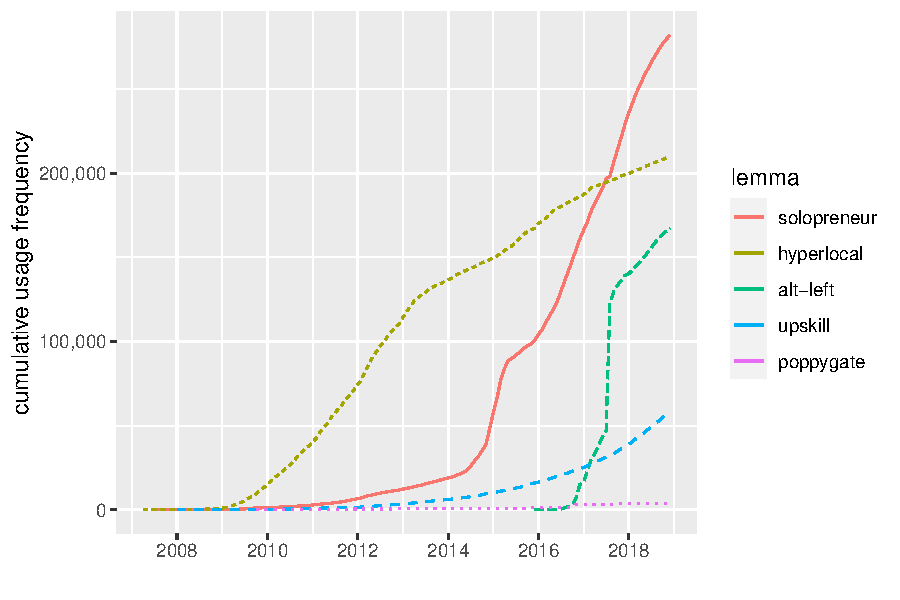
\includegraphics[width=\linewidth, height=.8\textheight, keepaspectratio]{../out/freq_cum_cases.pdf}
  \centering
  \end{figure}
  \footnotetext{For better visibility \ol{alt-right} was omitted from this plot because of its high usage frequency.}

  Most importantly,
  lifespan
  1 comparison: e.g. \ol{alt-left} vs. \ol{alt-right}

  introduce cases


  Potential distortions
  uses != users: This can distort the picture, e.g. if some speakers have a much stronger preference to use the term than the average or the amount of words contributed by by each speaker is not balanced.


  X is most frequent
  Y is oldest
  \ol{poppygate}

  \subsection{Temporal dynamics of usage intensity}

  instead of cumulative counts we now look at absolute frequency counts over time (in monthly bins)

  case studies

  \begin{figure}
  \caption{Temporal dynamics in usage frequency for case studies.}
  \centering
  \begin{subfigure}{.3\linewidth}
  \caption{\ol{upskill}}
  \includegraphics[width=\linewidth, height=.8\textheight, keepaspectratio]{"../out/uses/ui_upskill_time"}
  \end{subfigure}
  \begin{subfigure}{.3\linewidth}
  \caption{\ol{hyperlocal}}
  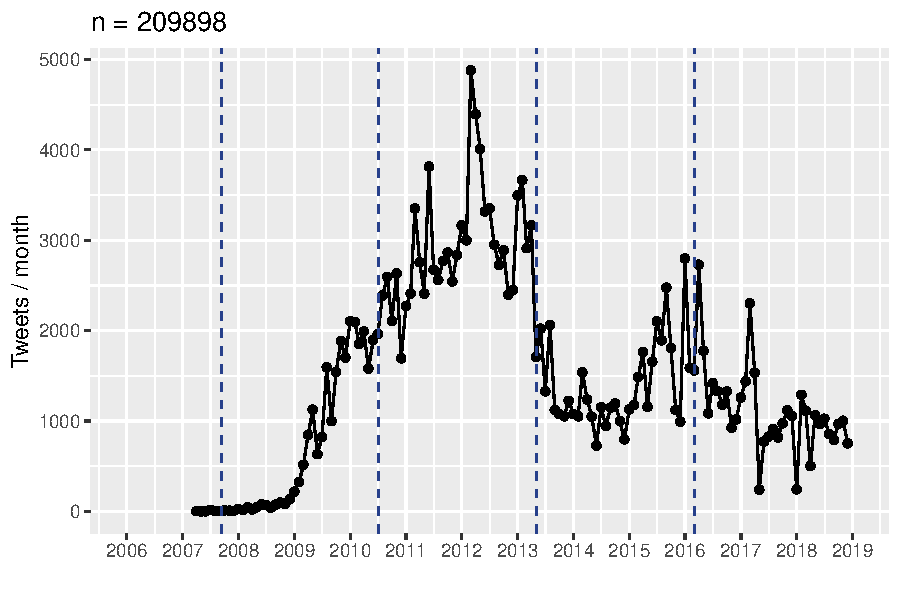
\includegraphics[width=\linewidth, height=.8\textheight, keepaspectratio]{../out/uses/ui_hyperlocal_time.pdf}
  \end{subfigure}
  \begin{subfigure}{.3\linewidth}
  \caption{\ol{solopreneur}}
  \includegraphics[width=\linewidth, height=.8\textheight, keepaspectratio]{"../out/uses/ui_solopreneur_time"}
  \end{subfigure}

  \begin{subfigure}{.3\linewidth}
  \caption{\ol{alt-right}}
  \includegraphics[width=\linewidth, height=.8\textheight, keepaspectratio]{"../out/uses/ui_alt-right_time"}
  \end{subfigure}
  \begin{subfigure}{.3\linewidth}
  \caption{\ol{alt-left}}
  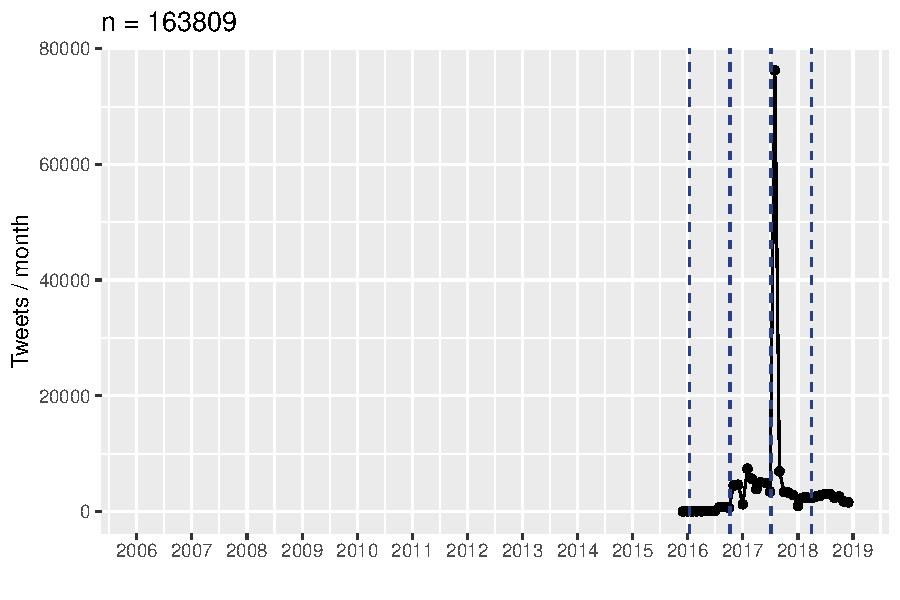
\includegraphics[width=\linewidth, height=.8\textheight, keepaspectratio]{../out/uses/ui_alt-left_time.pdf}
  \end{subfigure}
  \begin{subfigure}{.3\linewidth}
  \caption{\ol{poppygate}}
  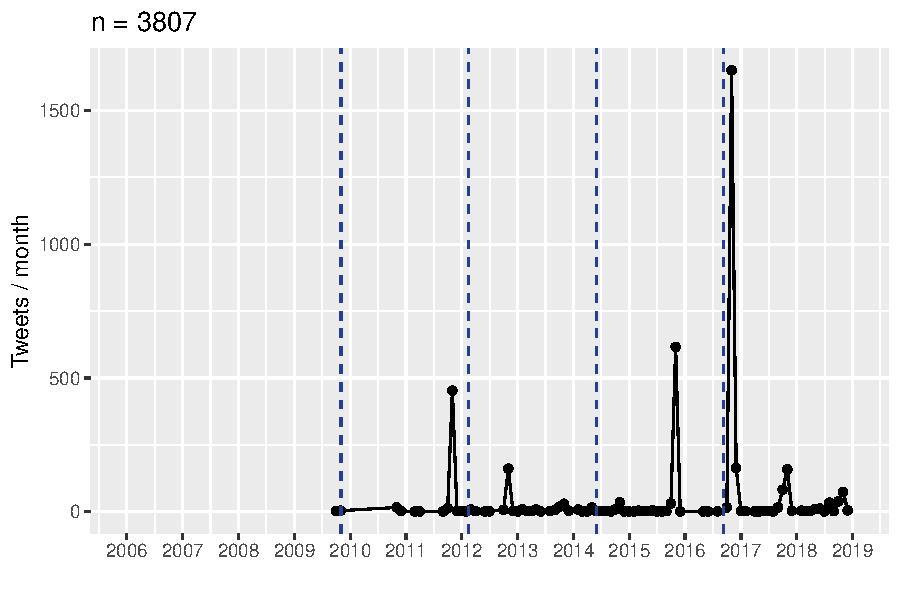
\includegraphics[width=\linewidth, height=.8\textheight, keepaspectratio]{../out/uses/ui_poppygate_time.pdf}
  \end{subfigure}
  \end{figure}

  different patterns
  stability
  trend
  speed of diffusion

  stability: shows that freq. is problematic
  \enquote{dormant}
  spikes distort representativity of frequency for degree of conventionality
  underestimate: \ol{poppygate} not forgotten in troughs
  overestimate: cumulating hides the fact that words like \ol{millenium} do get lost

  full sample

  coefficient of variation
  most volatile
  least volatile

  volatile patterns are the rule than the exception for \emph{lexical innovation}
  due to nature of \emph{lexical} innovation
  bound to cultural conceptual salience (variable \enquote{semantic carrying capacity}~\parencite{Nini2017ApplicationGrowth})
  needs to be accounted for

  trend
  increasing: looks successful
  decreasing: looks unsuccessful

  going beyond frequency
  In the following sections I will assess the value of usage frequency and compare and complement it with social network information about the diffusion of lexical innovations.

\section{Social networks of diffusion}

  \subsection{Centralization over time}

  going beyond frequency

  def. diffusion:
  numbers of users
  communities

  subsetting / time slices
  start of diffusion process
  4 quarters

  explain: degree centralization

  case studies

  example where freq. meets nets

  example where nets add to freq.: \ol{alt-left}

    \subsubsection{Overview of changes in centralization for case studies.}

  \begin{figure}[H]
  \caption{Degree centralization over time for case study words.}
  \centering
  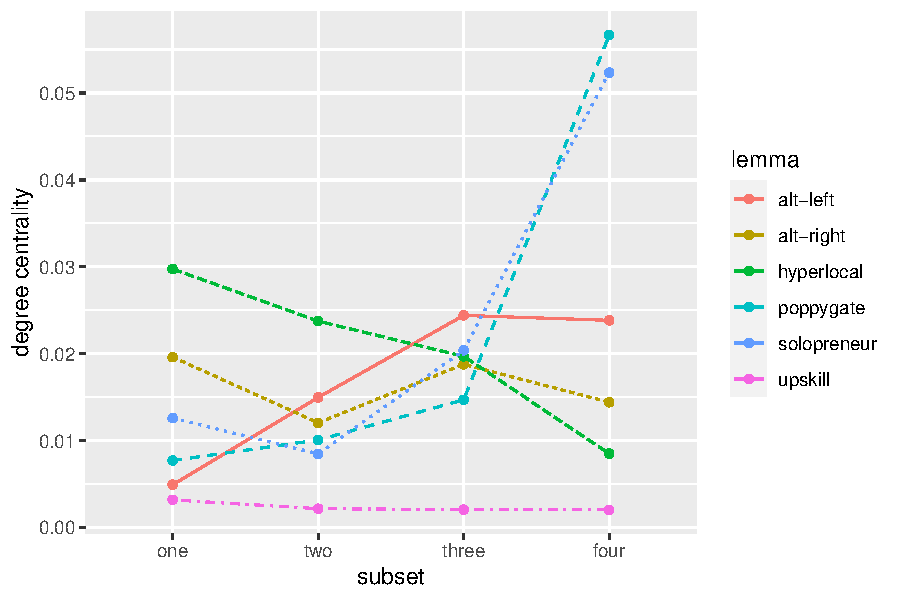
\includegraphics[width=\linewidth, height=.8\textheight, keepaspectratio]{../out/cases_cent_diac.pdf}
  \end{figure}

    \subsubsection{Advanced / increasing: \ol{hyperlocal}}

  \begin{figure}[H]
  \caption{Social network of diffusion for \ol{hyperlocal} over time.}
  \centering
  \begin{subfigure}{.45\linewidth}
  \caption{First stage}
  \centering
  \includegraphics[width=\linewidth, height=\textheight, keepaspectratio]{../gephi/plots/hyperlocal_one.pdf}
  \end{subfigure}
  \begin{subfigure}{.45\linewidth}
  \caption{Second stage}
  \centering
  \includegraphics[width=\linewidth, height=\textheight, keepaspectratio]{../gephi/plots/hyperlocal_two.pdf}
  \end{subfigure}\\
  \begin{subfigure}{.45\linewidth}
  \caption{Third stage}
  \centering
  \includegraphics[width=\linewidth, height=\textheight, keepaspectratio]{../gephi/plots/hyperlocal_three.pdf}
  \end{subfigure}
  \begin{subfigure}{.45\linewidth}
  \caption{Fourth stage}
  \centering
  \includegraphics[width=\linewidth, height=\textheight, keepaspectratio]{../gephi/plots/hyperlocal_four.pdf}
  \end{subfigure}
  \end{figure}

    \subsubsection{Limited / limited: \ol{alt-left}}

  \begin{figure}[H]
  \caption{Social network of diffusion for \ol{alt-left} over time.}
  \centering
  \begin{subfigure}{.45\linewidth}
  \caption{First stage}
  \centering
  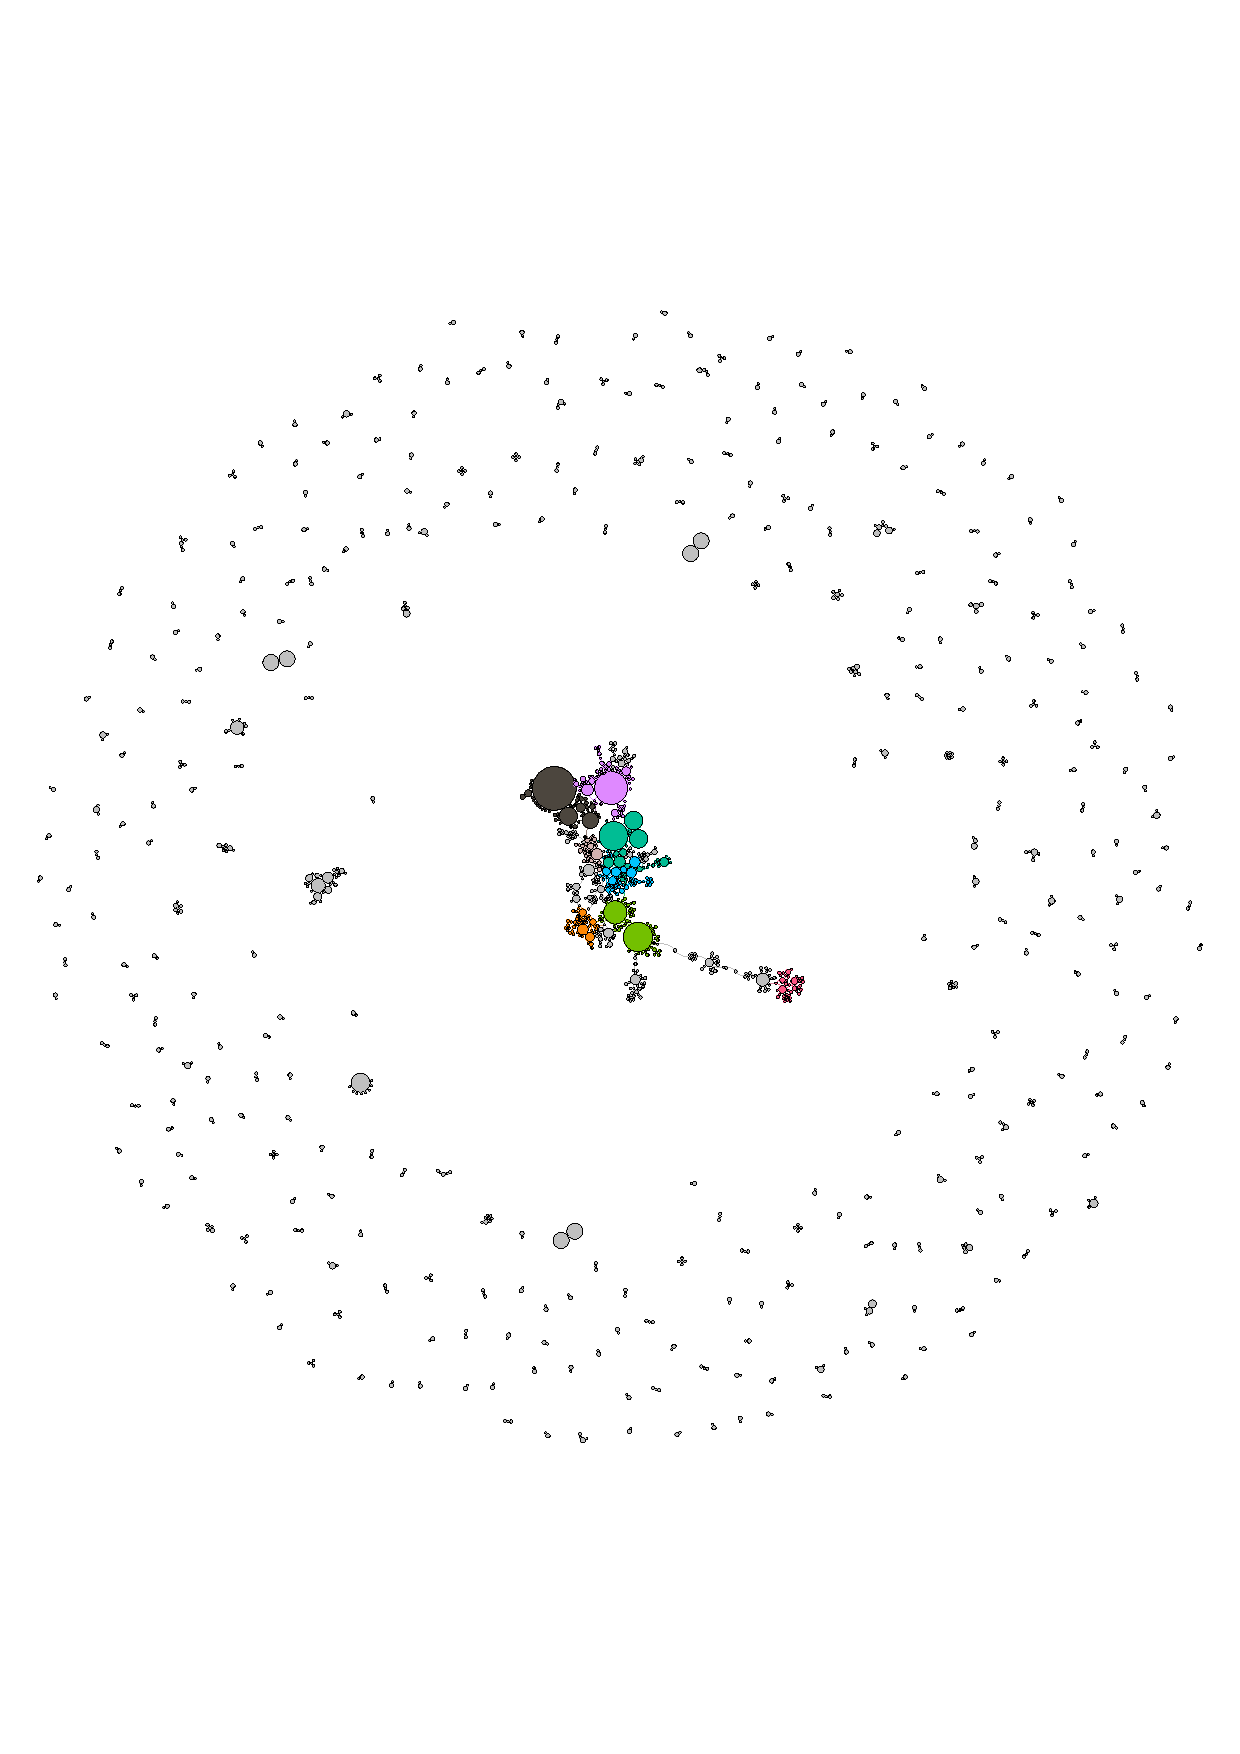
\includegraphics[width=\linewidth, height=\textheight, keepaspectratio]{../gephi/plots/alt-left_one.pdf}
  \end{subfigure}
  \begin{subfigure}{.45\linewidth}
  \caption{Second stage}
  \centering
  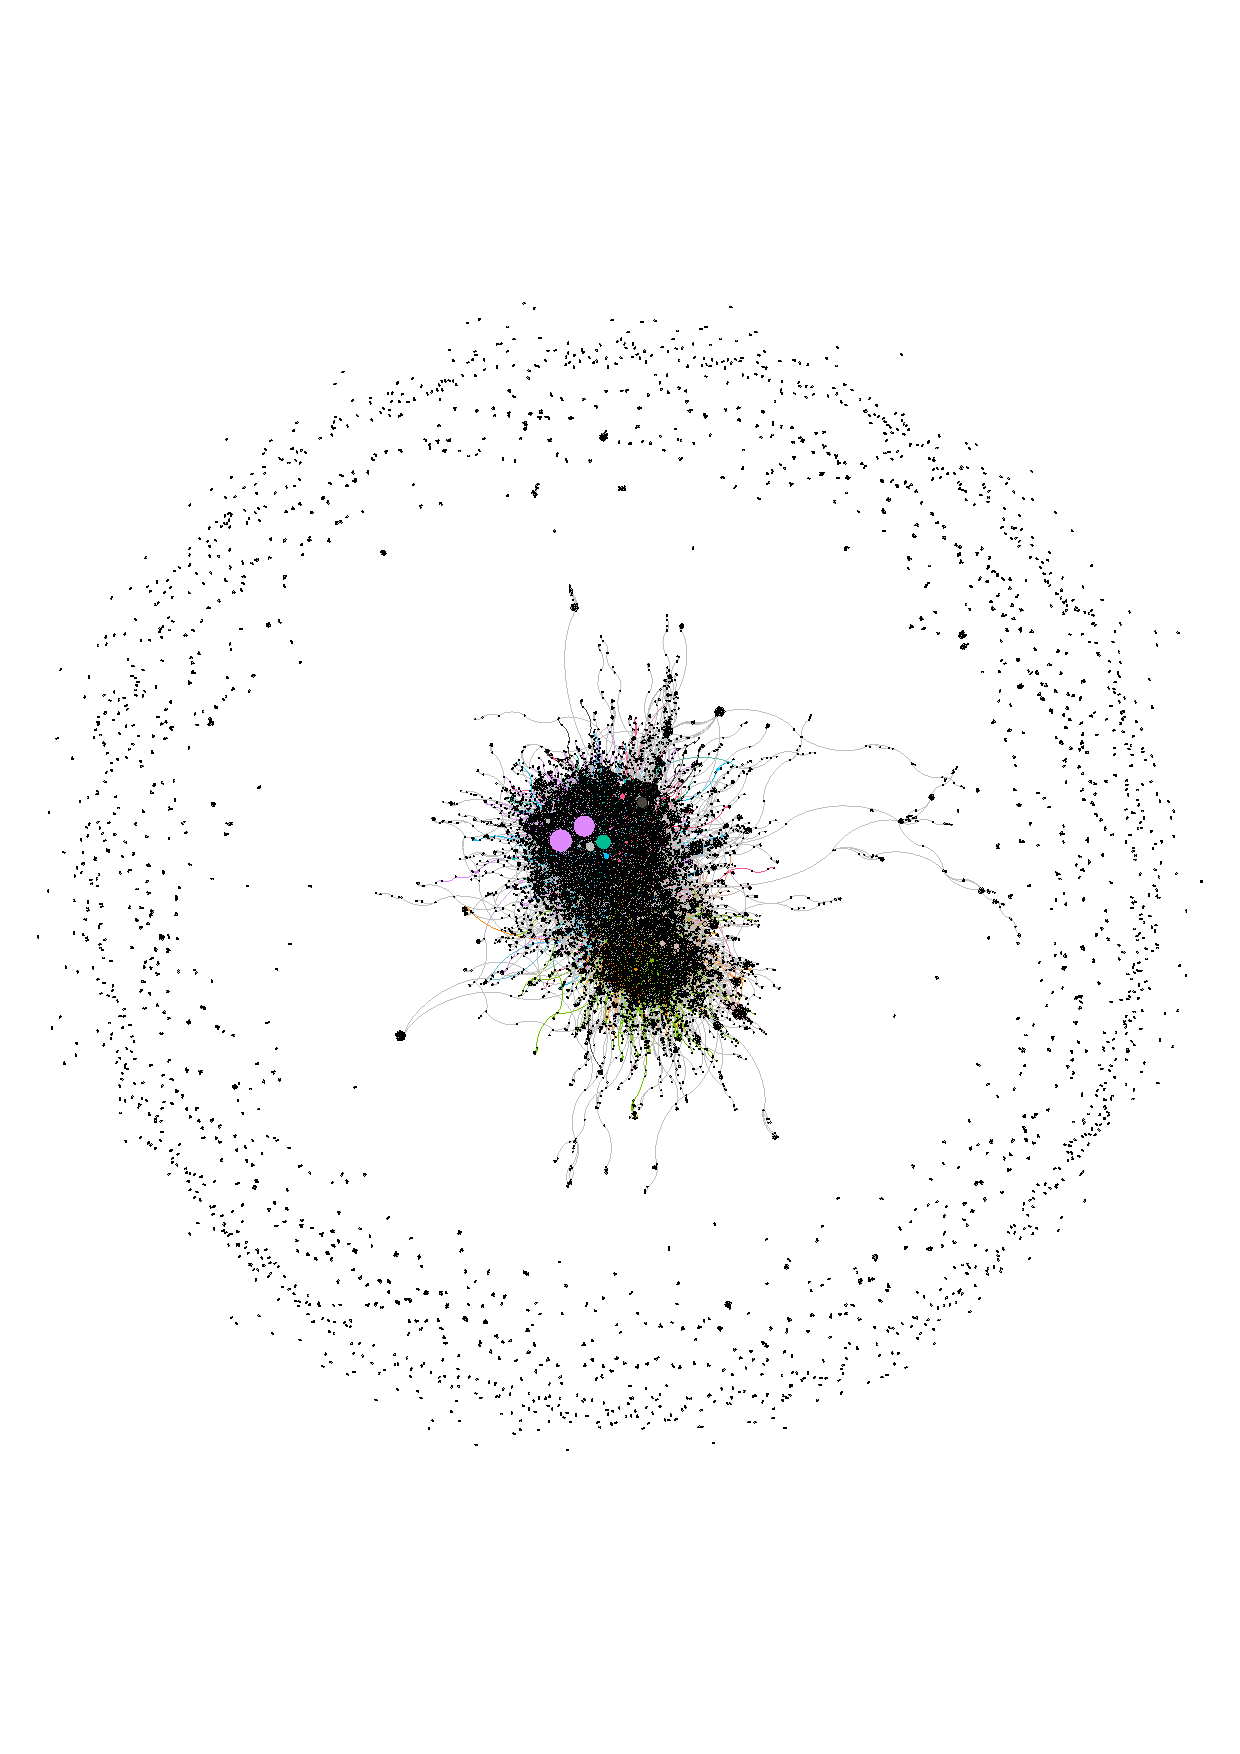
\includegraphics[width=\linewidth, height=\textheight, keepaspectratio]{../gephi/plots/alt-left_two.pdf}
  \end{subfigure}\\
  \begin{subfigure}{.45\linewidth}
  \caption{Third stage}
  \centering
  \includegraphics[width=\linewidth, height=\textheight, keepaspectratio]{../gephi/plots/alt-left_three.pdf}
  \end{subfigure}
  \begin{subfigure}{.45\linewidth}
  \caption{Fourth stage}
  \centering
  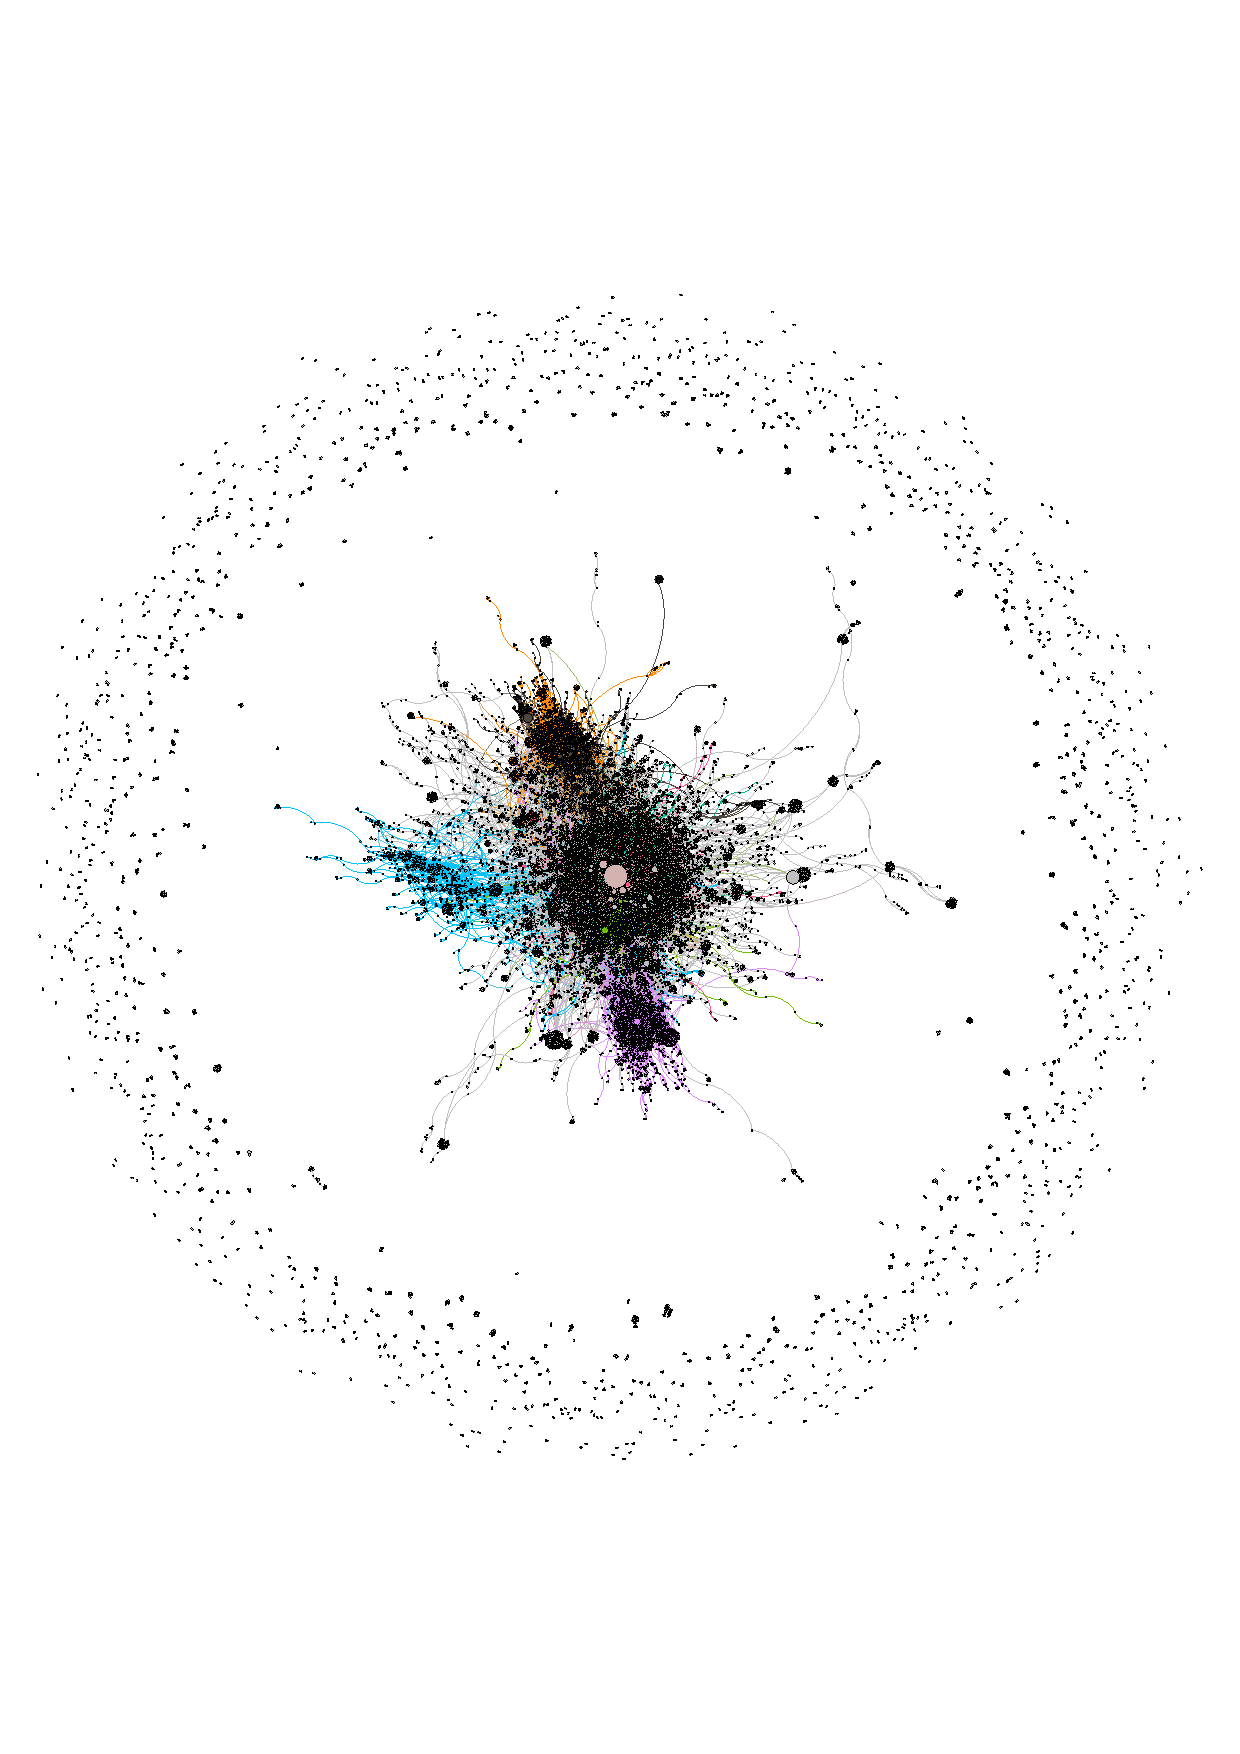
\includegraphics[width=\linewidth, height=\textheight, keepaspectratio]{../gephi/plots/alt-left_four.pdf}
  \end{subfigure}
  \end{figure}

    \subsubsection{Full sample}

  density
  successful
  unsuccessful

  biggest changes

  \subsection{Overall centralization}

  most diffused
  least diffused

\section{Networks vs. frequency}

  \subsection{Correlation}

  There is a significant correlation ($p = 0.015$) between frequency and centralization

  \subsection{Discrepancies}

  However, we also see discrepancies

  plots

  \begin{figure}[H]
  \centering
  \begin{subfigure}{.45\linewidth}
  \caption{Full sample.}
  \centering
  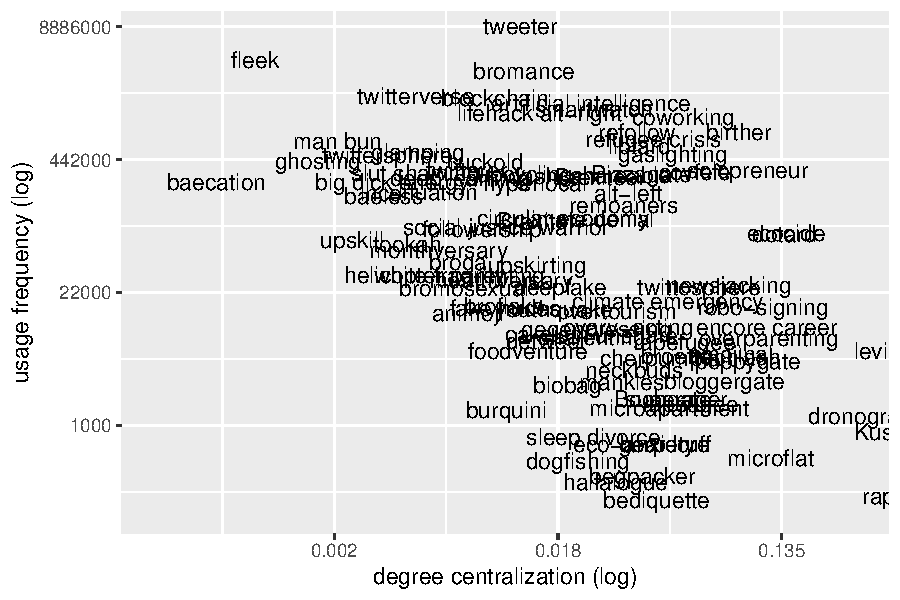
\includegraphics[width=\linewidth, height=.8\textheight, keepaspectratio]{../out/full_cent_freq_overall.pdf}
  \end{subfigure}
  \begin{subfigure}{.45\linewidth}
  \caption{Case studies.}
  \centering
  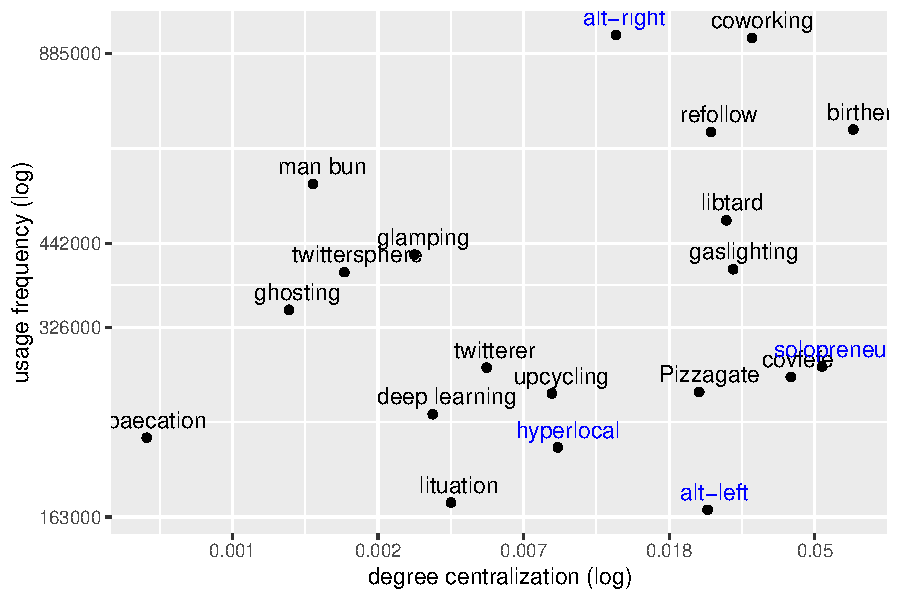
\includegraphics[width=\linewidth, height=.8\textheight, keepaspectratio]{../out/cases_cent_freq_overall.pdf}
  \end{subfigure}
  \end{figure}

  cluster analysis

  freq. overestimating
  topical
  propaganda: \ol{alt-right}, \ol{alt-left}, \ol{covfefe}, \ol{birther}
  Brexit terms: \ol{Brexiteer}, \ol{Brexiter}, \ol{Brexit}
  nerds
  technical

  freq. underestimating: XXX
  topical words

  Social network metrics certainly add to freq.

\section{Conclusion}

freq. proves to be a pretty good indicators
but
temporal dynamics important
social network dynamics important, esp. w.r.t. new words
cross-checking other data sources (NOW corpus) shows validity
social network analysis can be an important tool for sociolinguistics

%section{bibliography}

\printbibliography

\end{document}
